%%%%%%%%%%%%%%%%%%%%%%%%%%%%%%%%%%%%%%%%%%%%%%%%%%%%%%%%%%%%%%%%%%%%%%%%%%%%%%%%
%2345678901234567890123456789012345678901234567890123456789012345678901234567890
%        1         2         3         4         5         6         7         8

\documentclass[letterpaper, 10 pt, conference]{ieeeconf}  % Comment this line out if you need a4paper

%\documentclass[a4paper, 10pt, conference]{ieeeconf}      % Use this line for a4 paper

\IEEEoverridecommandlockouts                              % This command is only needed if 
                                                          % you want to use the \thanks command

\overrideIEEEmargins                                      % Needed to meet printer requirements.

%In case you encounter the following error:
%Error 1010 The PDF file may be corrupt (unable to open PDF file) OR
%Error 1000 An error occurred while parsing a contents stream. Unable to analyze the PDF file.
%This is a known problem with pdfLaTeX conversion filter. The file cannot be opened with acrobat reader
%Please use one of the alternatives below to circumvent this error by uncommenting one or the other
%\pdfobjcompresslevel=0
%\pdfminorversion=4

% See the \addtolength command later in the file to balance the column lengths
% on the last page of the document

% The following packages can be found on http:\\www.ctan.org
\usepackage{graphics} % for pdf, bitmapped graphics files
%\usepackage{epsfig} % for postscript graphics files
%\usepackage{mathptmx} % assumes new font selection scheme installed
%\usepackage{times} % assumes new font selection scheme installed
\usepackage{amsmath} % assumes amsmath package installed
\DeclareMathOperator*{\argmin}{\arg\!\min}

\usepackage{amssymb}  % assumes amsmath package installed
\usepackage{algorithmic}

\title{\LARGE \bf
Sparse, Predictive, and Interpretable Functional Connectomics with UoI$_{\text{Lasso}}$
}


\author{
    Pratik S. Sachdeva$^{1, 3}$, Sharmodeep Bhattacharyya$^{5}$, Kristofer E. Bouchard$^{1,2,3,4*}$%
    \thanks{
        $^{1}$Redwood Center for Theoretical Neuroscience, UC Berkeley
    }%
    \thanks{
        $^{2}$Helen Wills Neuroscience Institute, UC Berkeley
    }
    \thanks{
        $^{3}$Biological Systems \& Engineering, Lawrence Berkeley National Lab
    }
    \thanks{
        $^{4}$Computational Resources Division, Lawrence Berkeley National Lab
    }%
    \thanks{
        $^{5}$Department of Statistics, Oregon State University
    }
    \thanks{
        $^*$Corresponding author
    }%
}


\begin{document}



\maketitle
\thispagestyle{empty}
\pagestyle{empty}


%%%%%%%%%%%%%%%%%%%%%%%%%%%%%%%%%%%%%%%%%%%%%%%%%%%%%%%%%%%%%%%%%%%%%%%%%%%%%%%%
\begin{abstract}

Network formation from neural activity is a foundational problem in systems neuroscience. Functional networks, after downstream analysis, can provide key insights into the nature of neurobiological structure and computation. The validity of such insights hinges on accurate selection and estimation of the informative features.  However, commonly used statistical inference procedures generally fail to identify the correct features, and further introduce consequential bias in the estimates. To address these issues, we developed Union of Intersections (UoI), a flexible, modular, and scalable framework for enhanced statistical feature selection and estimation. Methods based on UoI perform feature selection and feature estimation through intersection and union operations, respectively. In the context of linear regression (specifically UoI$_{\text{Lasso}}$), we summarize extensive numerical investigation on synthetic data to demonstrate tight control of false-positives and false-negatives in feature selection with low-bias and low-variance estimates of selected parameters, while maintaining high-quality prediction accuracy. We demonstrate, with UoI$_{\text{Lasso}}$, the extraction of sparse, predictive, and interpretable functional networks from human electrocorticography recordings during speech production and  the inference of parsimonious coupling models from nonhuman primate single-unit recordings during reaching tasks. Our results establish that UoI$_{\text{Lasso}}$ generates interpretable and predictive functional connectivity networks.

\end{abstract}


%%%%%%%%%%%%%%%%%%%%%%%%%%%%%%%%%%%%%%%%%%%%%%%%%%%%%%%%%%%%%%%%%%%%%%%%%%%%%%%%
\section{INTRODUCTION}
The increasing size and complexity of neuroscientific and biomedical data could dramatically enhance basic discovery and prediction. Realizing this potential requires novel statistical analysis methods that are both interpretable and predictive. By \textit{interpretable}, we mean that one can interpret the output of the method in terms of processes generating the data. This typically requires identification of a small number of elements of the actual data (i.e., sparsity, Fig. \ref{fig:intro}a) and accurate estimation of their contribution (i.e., low-bias and low-variance, Fig. \ref{fig:intro}b). By \textit{predictive}, we mean optimizing the performance of some machine learning measure such as precision, recall, etc. There is often a trade-off between interpretability and predictive power, and methods that satisfy both are lacking. This tradeoff is particularly acute for neuroscientific applications, where the output of the model is used to provide insight into neurobiological functions. 

An important neuroscientific application that requires both predictive and interpretable statistical analysis is network estimation from data (i.e., ``functional connectomics'') \cite{fc}. In functional connectomics, statistical relationships between constituent units (e.g., neurons or electrodes) are quantified and expressed as graphs (Fig. \ref{fig:functional_coupling}). Downstream analyses can be performed on such graphs to elucidate the structure of the underlying physical mechanisms (e.g., the nature of neural computation) \cite{bassett}. Thus, accurate extraction of the network itself, which requires precise selection (i.e., identifying the non-zero edges), is of paramount importance. While \textit{ad-hoc} thresholding can be performed, such approaches are often set by hand and defy rigorous understanding. Likewise, statistically biased estimates can result in incorrectly inferred dynamics or under-estimated spike rates. These issues are fundamental to many neuroscientific data analyses and the interpretation thereof.

\begin{figure}[b]
    \vspace{-15pt}
    \centering
    \scalebox{0.54}{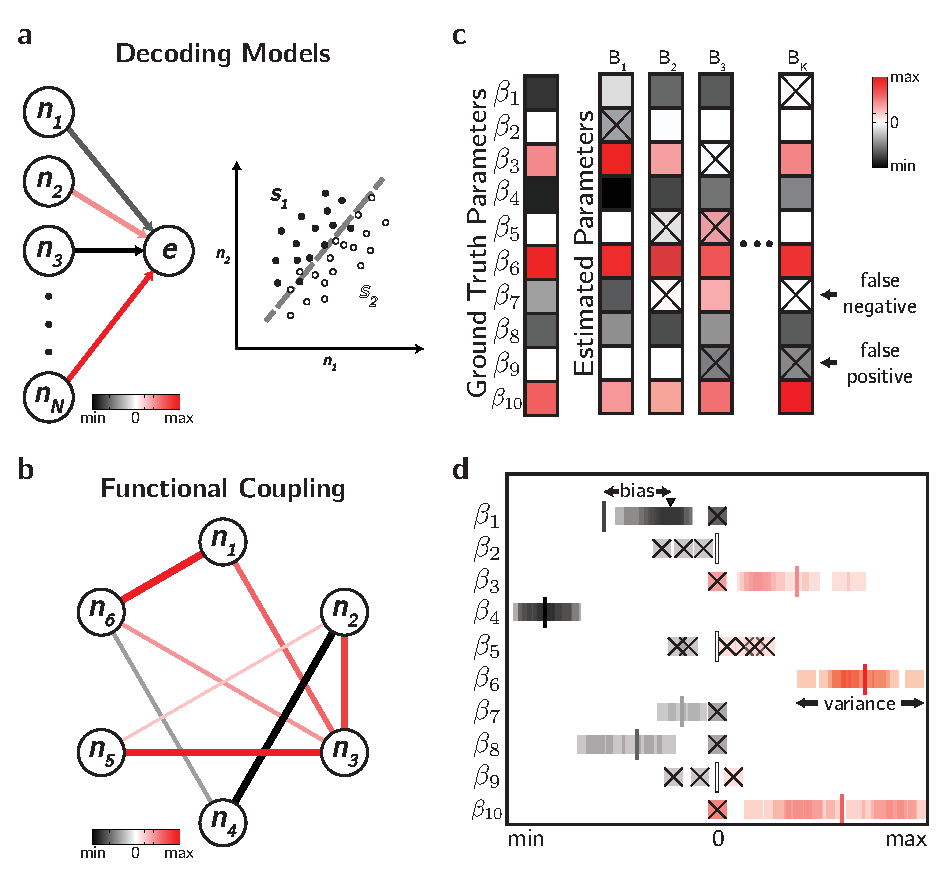
\includegraphics{./img/Fig1/Fig1}}
    \vspace{-20pt}
    \caption{Estimation of ground truth parameters over resamples of the data ($R_i$). \textbf{a.} Poor selection results in false positives and false negatives. \textbf{b.} Poor estimation results in high bias and high variance.}
    \label{fig:intro}
\end{figure}

We present the Union of Intersections (UoI) framework, a novel statistical approach we have recently introduced that addresses these issues \cite{uoi}. Algorithms enhanced by UoI (e.g., regression, classification, dimensionality reduction) are ubiquitous in systems neuroscience. Here, we apply the UoI framework to Lasso regression in order to extract sparse, predictive, and interpretable functional networks from neuroscience datasets. We demonstrate qualitatively and quantitatively different results when using UoI$_{\text{Lasso}}$  compared to ``standard'' methods.  Thus, the foundational statistical improvements of UoI-based methods will potentially have significant impacts across neuroscience.

\section{METHODS}
\subsection{Human Electrocorticography}
We considered a dataset (Chang lab) comprised of electrocorticography (ECoG) recordings (86 electrodes) taken directly from the surface of the ventral sensory-motor cortex (vSMC) in human brain during speech production (45 trials each) \cite{bouchard2013}. The subject read aloud consonant-vowel syllables (CVs) composed of 19 consonants followed by one of three vowels (/a/, /i/ or /u/). Each CV was produced between 15 and 100 times total.  We utilized the $z$-scored (to baseline activity) H$\gamma$ analytic amplitude extracted from the cortical field potentials.

\subsection{Nonhuman Primate Single-Unit Activity}
The second dataset (Sabes lab) contains simultaneously recorded single-unit activity in primary motor cortex (M1) of Macaque monkey (196 single-units) \cite{nhp}. The behavioral task consisted of self-paced reaches to targets arranged in a grid without gaps or pre-movement delay intervals. We binned spike counts at 500 milliseconds and applied a square-root transform to stabilize the variance (1716 samples).

\begin{figure}[t]
    \centering
    \scalebox{0.95}{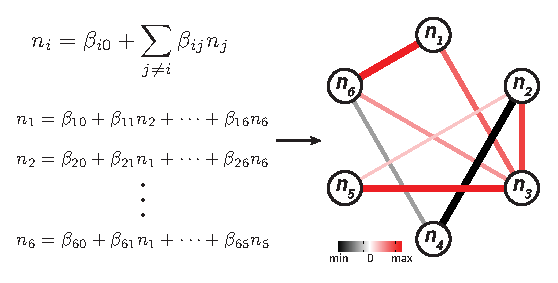
\includegraphics{./img/Fig2/Fig2}}
    \vspace{-10pt}
    \caption{\textbf{Left:} Functional coupling models express the activity of a neuron/electrode as a function of neighboring neurons/electrodes (e.g., linear models). \textbf{Right:} Coupling models can generate partial correlation graphs.}
    \label{fig:functional_coupling}
    \vspace{-15pt}
\end{figure}

\subsection{ UoI$_{\text{Lasso}}$ and Linear Regression}
UoI is not a single method or algorithm but a flexible statistical framework into which other algorithms can be inserted. UoI-based methods leverage stochastic data resampling and a range of sparsity-inducing regularization parameters to build families of potential feature sets robust to perturbations (i.e., resamples) of the data, and then average nearly unbiased parameter estimates of selected features to maximize predictive accuracy. In this work, we focus on the UoI framework applied to Lasso regression, or UoI$_{\text{Lasso}}$.

Linear regression consists of estimating the parameters $\beta \in \mathbb{R}^p$ that map a $p$-dimensional vector of predictor variables $x \in \mathbb{R}^p$ to the observation variable $y\in \mathbb{R}$, when the $n$ samples are corrupted by i.i.d Gaussian noise:
$$
y = \beta^T x + \epsilon
$$
where $\epsilon \sim \mathcal{N}(0, \sigma^2)$ for each sample. When the true $\beta$ is thought to be sparse, an estimate of $\beta$ (i.e., $\hat{\beta}$) can be found by solving a constrained optimization problem of the form
$$
\hat{\beta} \in \underset{\beta\in \mathbb{R}^p}{\text{argmin}} \sum_{i=1}^n(y_i - \beta x_i)^2 + \lambda |\beta|_1
$$
where $|\beta|_1$ is the $\ell_1$-norm of the parameters (i.e., the Lasso). Typically, $\lambda$ is unknown and must be determined through cross-validation across a set of hyperparameters $\left\{\lambda_j\right\}_{j=1}^k$.

The key mathematical idea underlying UoI is to perform
model selection through intersection (compressive) operations and model estimation through union (expansive) operations, in that order. For UoI$_{\text{Lasso}}$, the procedure is as follows:
\begin{itemize}
    \item \textbf{Model Selection:} For each $\lambda_j$, generate Lasso estimates on $N_S$ resamples of the data. The support $S_j$ (i.e., the set of non-zero parameters) for $\lambda_j$ consists of the features that persist in all model fits across the resamples (Fig. \ref{fig:uoi}, top left).
    \item \textbf{Model Estimation:} For each support $S_j$, perform Ordinary Least Squares (OLS) on $N_E$ resamples of the data. The final model is obtained by averaging across the supports that optimally predict held-out data for each resample (Fig. \ref{fig:uoi}, top right). 
\end{itemize}
Thus, the selection module ensures that, for each $\lambda_j$, only features that are stable to perturbations in the data (resamples) are allowed in the support $S_j$. Meanwhile, the estimation module ensures that only the predictive supports are averaged together in the final model. The degree of feature compression via intersections (quantified by $N_S$) and the degree of feature expansion via unions (quantified by $N_E$) can be balanced to maximize prediction accuracy for the response variable $y$.

We consider functional coupling models where the activity of a unit can be expressed as a linear combination of its neighbors' activities (Fig. \ref{fig:functional_coupling}, left). The fitted parameters obtained from these models can be used to generate networks, such as partial correlation graphs (Fig. \ref{fig:functional_coupling}, right).
\begin{figure}[t]
    \centering
    \scalebox{0.50}{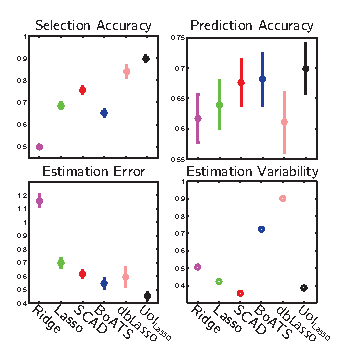
\includegraphics{./img/Fig3/Fig3}}
    \vspace{-10pt}
    \begin{algorithmic}[1]
        \renewcommand{\algorithmicrequire}{\textbf{Input:}}
        \renewcommand{\algorithmicensure}{\textbf{Output:}}
        \REQUIRE Data $X \in \mathbb{R}^{n\times p}$, $y \in \mathbb{R}^{n}$
        \STATE \ \ \ \  Regularization strengths $\lambda \in \mathbb{R}^q$
        \STATE \ \ \ \  Number of resamples $N_S$ and $N_E$
        \STATE \ \ \ \  Loss function $L(\beta; X, y)$
        \STATE \textit{Model Selection}
        \FOR {$k = 1$ to $N_S$}
            \STATE Generate resample $X^k$, $y^k$
            \FOR {$\lambda_j \in \lambda$}
                \STATE $\hat{\beta}^{jk}\leftarrow$ Lasso regression (penalty $\lambda_j$) of $y^k$ on $X^k$
                \STATE $S_j^k \leftarrow \left\{i\right\}$ where $\hat{\beta}^{jk}_i \neq 0$
            \ENDFOR
        \ENDFOR
        \FOR {$j = 1$ to $q$}
            \STATE $\displaystyle S_j \leftarrow \bigcap_{k=1}^{N_S}S_j^k$ \hfill $\triangleright$ \textit{ Intersection}
        \ENDFOR
        \STATE \textit{Model Estimation}
        \FOR {$k=1$ to $N_B$}
            \STATE Generate training $\left(X_T^k, y_T^k\right)$ and evaluation $\left(X_E^k, y_E^k\right)$ resamples
            \FOR {$j=1$ to $q$}
                \STATE $X_{T, j}^k, X_{E, j}^k \leftarrow $ $X_T^k, X_E^k$ with features $S_j$ extracted. 
                \STATE $\hat{\beta}^{jk} \leftarrow$ OLS Regression of $y_T^k$ on $X_{T,j}^k$
                \STATE $\ell^{jk} \leftarrow L(\hat{\beta}^{jk}; X^k_{E, j}, y_E^k)$
            \ENDFOR
            \STATE $\hat{\beta}^k \leftarrow \underset{\hat{\beta}^{jk}}{\argmin} \ \ell^{jk}$
        \ENDFOR
        \STATE $\hat{\beta}^* = \underset{k}{\text{median}}\left(\hat{\beta}_k\right)$ \hfill $\triangleright$ \textit{ Union}
        \RETURN $\hat{\beta}^*$ 
    \end{algorithmic} 
    \vspace{-8pt}
    \caption{\textbf{Top:} Schematic depicting the Union of Intersections framework applied to Lasso. \textbf{Bottom:} Pseudocode for UoI$_{\text{Lasso}}$}
    \label{fig:uoi}
    \vspace{-15pt}
\end{figure}

\subsection{Metrics}
We evaluated all algorithms with the following metrics:
\begin{itemize}
    \item \textbf{Selection Accuracy:} $1-\frac{\vert S_{\hat{\beta}} \Delta S_{\beta}\vert}{|S_{\hat{\beta}}\vert + \vert S_{\beta} \vert}$, where $\Delta$ is the symmetric set difference operator and $|S|$ is the cardinality of $S$. This metric is bounded in $[0, 1]$, taking value $0$ if $S_{\hat{\beta}}$ and $S_{\beta}$ have no elements in common, and taking value $1$ iff they are identical.
    \item \textbf{Selection Ratio:} The fraction of parameters fitted to be non-zero. Alternatively, we refer to the model size, or the number of fitted non-zero features.
    \item \textbf{Estimation Error:} $\sqrt{\frac{1}{p} \sum (\beta_i - \hat{\beta}_i)^2}$ (i.e., rms error).
    \item \textbf{Estimation Variability:} $\text{var}[\hat{\beta}]$, taken across resamples.
    \item \textbf{Prediction Accuracy:} $\frac{\sum \left(y_i - \hat{y}_i\right)^2}{\sum \left(y_i - E[y]\right)^2}$ (i.e., $R^2$).
    \item \textbf{Model Parsimony:} Bayesian Information Criterion (BIC), defined as $\text{BIC} = -2\log \hat{L} + |\hat{\beta}|_0 \log(n)$, where $\hat{L}$ is the likelihood of the test set and $|\cdot|_0$ denotes the $\ell_0$-norm. Lower BIC, indicative of a predictive model using fewer features, is preferred.
\end{itemize}

\section{RESULTS}
\subsection{Simulated Datasets}
To demonstrate the performance of the UoI$_{\text{Lasso}}$ algorithm, we performed extensive numerical investigations on simulated data sets, where we controlled key properties of the data. We benchmarked UoI$_{\text{Lasso}}$ against five other selection/estimation methods: Ridge \cite{elements}, Lasso \cite{lasso}, Smoothly Clipped Absolute Deviation (SCAD) \cite{scad}, Boostrapped Adaptive Threshold Selection (BoATS) \cite{boats}, and debiased Lasso \cite{dbLasso}. 

We examined the performance of these algorithms across a variety of underlying distributions of model parameters, degrees of sparsity, and noise levels. In Figure \ref{fig:uoi}, we present our results on an experiment with 300 total parameters and 100 non-zero parameters symmetrically distributed with exponential increasing frequency as a function of parameter magnitude. The metrics displayed are taken across 100 randomized cross-validation samples of the data. We found that UoI$_{\text{Lasso}}$ (Fig. \ref{fig:simulated}, black) possessed the highest selection accuracy (Fig. \ref{fig:simulated}a), lowest estimation error (Fig. \ref{fig:simulated}b), best prediction accuracy (Fig \ref{fig:simulated}c), and superior estimation variability (Fig. \ref{fig:simulated}d). Additionally, UoI$_{\text{Lasso}}$'s high selection accuracy manifested as the most accurate model size (Fig. \ref{fig:simulated}e), which, in combination with its prediction accuracy, resulted in the best model parsimony (Fig. \ref{fig:simulated}f). Overall, UoI$_{\text{Lasso}}$ was robust to differences in underlying parameter distribution, degree of sparsity, and magnitude of noise \cite{uoi}.
\begin{figure}[t]
    \centering
    \scalebox{1.05}{\includegraphics{./img/Fig4/Fig4}}
    \vspace{-20pt}
    \caption{Performance of UoI (black) compared to other models (in order: Ridge, Lasso, SCAD, BoATS, debiased Lasso) on simulated data.}
    \label{fig:simulated}
    \vspace{-15pt}
\end{figure}

\subsection{Functional Networks from Human Neural Recordings}

We sought to determine if the enhanced selection and estimation properties of UoI$_{\text{Lasso}}$ translated into its utility as a tool for data-driven discovery in complex neuroscience data sets. We constructed sparse neuroscientifically-meaningful partial correlation graphs (using the functional coupling models in Fig. 2) from the human ECoG recordings. The model was estimated independently for each electrode, and we benchmarked UoI$_{\text{Lasso}}$ with SCAD. In Fig. \ref{fig:vsmc}a-b, we display the networks derived from recordings during the production of /b/ while speaking /ba/. We found that the UoI$_{\text{Lasso}}$ network (Fig. \ref{fig:vsmc}a) was much sparser than the SCAD network (Fig. \ref{fig:vsmc}b). Furthermore, the network extracted by UoI$_{\text{Lasso}}$ contained electrodes in the lip (dorsal vSMC), jaw (central vSMC), and larynx (ventral vSMC) regions, accurately reflecting the articulators engaged in the production of /b/ (Fig. \ref{fig:vsmc}c). The SCAD network (Fig. \ref{fig:vsmc}d) did not have any of these properties. This highlights the improved power of UoI$_{\text{Lasso}}$ to extract sparse graphs with functionally meaningful features relative to even some non-convex methods.

We calculated connectivity graphs during the production of 9 consonant-vowel syllables. Fig. \ref{fig:vsmc}e displays a summary of prediction accuracy for UoI$_{\text{Lasso}}$ networks (red) and SCAD networks (black) as a function of time. The average relative prediction accuracy (compared to baseline times) for the UoI$_{\text{Lasso}}$ network was generally greater during the time of peak phoneme encoding ($T = \left[-100:200\right]$) compared to the SCAD network. Fig. \ref{fig:vsmc}f plots the time course of the parameter selection ratio for the UoI$_{\text{Lasso}}$ network (red) and SCAD network (black). The UoI$_{\text{Lasso}}$ network was consistently 5 times sparser than the SCAD network. These results demonstrate that UoI$_{\text{Lasso}}$ extracts sparser graphs from noisy neural signals with a modest increase in prediction accuracy compared to SCAD.

\begin{figure}[t]
    \centering
    \scalebox{0.80}{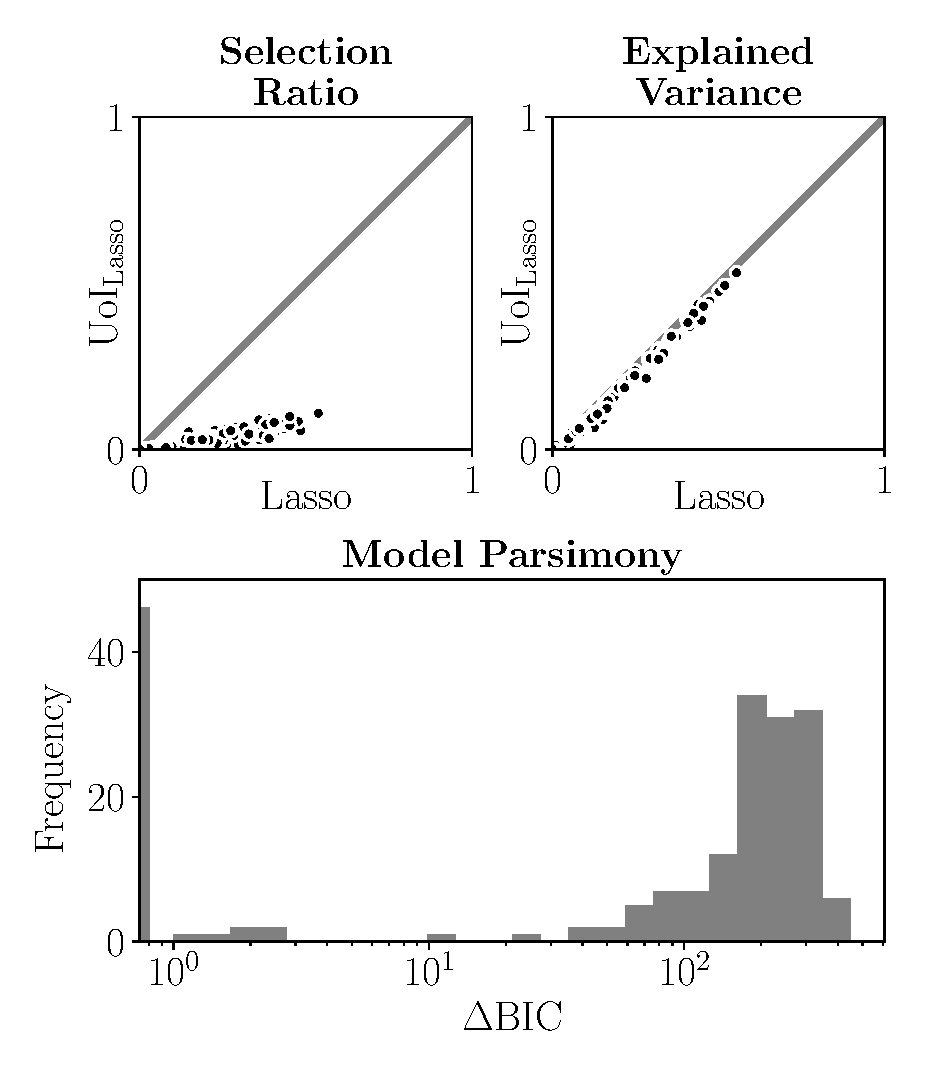
\includegraphics{./img/Fig5/Fig5}}
    \vspace{-10pt}
    \caption{\textbf{a, b.} Partial correlation graphs obtained from UoI$_{\text{Lasso}}$ and SCAD, respectively. \textbf{c, d.} The locations of the electrodes on vSMC. \textbf{e.} Average relative (to baseline) prediction accuracy during the production of a CV syllable. \textbf{f} Average selection ratio over the same time course.}
    \label{fig:vsmc}
    \vspace{-15pt}
\end{figure}

\subsection{Sparse and Predictive Coupling Models from Nonhuman Primate Single-Unit Activity}
A significant strength of UoI$_{\text{Lasso}}$ is its ability to accurately deduce the true model size. Our simulations revealed that several standard approaches have a propensity to exaggerate the number of non-zero parameters (i.e., generate false positives: Fig. \ref{fig:simulated}e). In coupling models, such false positives may problematically imply the existence of functional sub-networks that do not exist. Thus, we examined whether, on an additional dataset, UoI$_{\text{Lasso}}$ is able to extract more parsimonious models, demonstrating that standard methods overstate the number of functional connections.

We computed coupling models on the 196 nonhuman primate M1 single-units, using  Lasso and UoI$_{\text{Lasso}}$. UoI$_{\text{Lasso}}$ provided considerably sparser fits (Fig. \ref{fig:nhp}a). On average, UoI$_{\text{Lasso}}$ used 8 times fewer parameters than Lasso. However, UoI$_{\text{Lasso}}$ maintained the predictive quality across all the fits (Fig. \ref{fig:nhp}b). These two observations can be summarized succinctly with the BIC. The difference in BIC $(\Delta$BIC = BIC$_{\text{Lasso}}-$BIC$_{\text{UoI}})$ across the model fits is depicted in Fig. \ref{fig:nhp}c. Approximately a quarter of the fits exhibit almost no difference in BIC, indicating there is little evidence against the models provided by Lasso.  Meanwhile, about 70\% of the single-units have a difference in BIC of at least 10, indicating very strong evidence against Lasso as a descriptive model of the data \cite{kass1995}. Thus, UoI$_{\text{Lasso}}$ provides coupling networks that are as simple as possible, but no simpler. 

\section{CONCLUSION}

UoI-based methods leverage stochastic data resampling and a range of sparsity-inducing regularization parameters/dimensions to build families of potential features, and then average nearly unbiased parameter estimates of selected features to maximize predictive accuracy. Thus, UoI separates model selection with intersection operations from model estimation with union operations: the limitations of selection by intersection are counteracted by the union of estimates, and vice versa. Stochastic data resampling can be a viewed as a perturbation of the data, and UoI efficiently identifies and robustly estimates features that are stable to these perturbations. Here, using UoI$_{\text{Lasso}}$, we demonstrated that these properties result in superior selection and estimation performance on simulated data as well as the generation of sparse, interpretable models on neuroscience datasets.

\begin{figure}[t]
    \centering
    \scalebox{0.38}{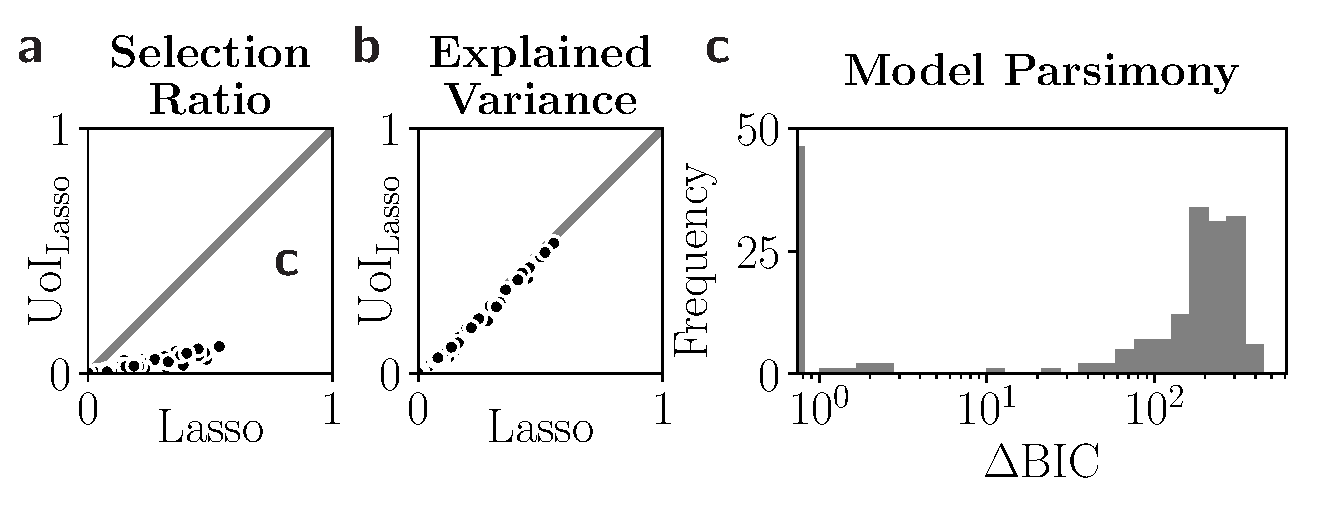
\includegraphics{./img/Fig6/Fig6}}
    \vspace{-15pt}
    \caption{UoI$_{\text{Lasso}}$ generates more parsimonious coupling models of single-unit activity. \textbf{a.} Comparison of selection ratios across the 196 coupling fits. \textbf{b.} Comparison of (cross-validated) $R^2$ values for each coupling fit. \textbf{c.} Comparison of BIC across model fits ($\Delta\text{BIC}=\text{BIC}_{\text{Lasso}} - \text{BIC}_{\text{UoI}}$).}
    \label{fig:nhp}
    \vspace{-15pt}
\end{figure}

In this work, we focused on neuroscience applications of UoI$_{\text{Lasso}}$. However, other machine learning algorithms fit naturally in the UoI framework. For example, we have successfully developed  the UoI$_{\text{Logistic}}$, UoI$_{\text{Poisson}}$, UoI$_{\text{VAR}}$, UoI$_{\text{CUR}}$, and UoI$_{\text{NMF}}$ algorithms and applied them to neuroscience datasets (e.g., \cite{uoi}). In addition, UoI has a high degree of natural algorithmic parallelism that we have exploited in a distributed Python-MPI implementation. With the diversity of use cases and ease of application to large datasets, UoI has the potential to provide data-driven insight in a variety of neuroscientific and biomedical contexts.

\addtolength{\textheight}{-12cm}   % This command serves to balance the column lengths
                                  % on the last page of the document manually. It shortens
                                  % the textheight of the last page by a suitable amount.
                                  % This command does not take effect until the next page
                                  % so it should come on the page before the last. Make
                                  % sure that you do not shorten the textheight too much.

%%%%%%%%%%%%%%%%%%%%%%%%%%%%%%%%%%%%%%%%%%%%%%%%%%%%%%%%%%%%%%%%%%%%%%%%%%%%%%%%



%%%%%%%%%%%%%%%%%%%%%%%%%%%%%%%%%%%%%%%%%%%%%%%%%%%%%%%%%%%%%%%%%%%%%%%%%%%%%%%%



%%%%%%%%%%%%%%%%%%%%%%%%%%%%%%%%%%%%%%%%%%%%%%%%%%%%%%%%%%%%%%%%%%%%%%%%%%%%%%%%

\section*{ACKNOWLEDGMENT}

P.S. Sachdeva was supported by the Department of Defense (DoD) through the National Defense Science \& Engineering Graduate Fellowship (NDSEG) Program. K.E. Bouchard was funded by a DOE/LBNL LDRD, ``Deep Learning for Science'', (PI, Prabhat).


%%%%%%%%%%%%%%%%%%%%%%%%%%%%%%%%%%%%%%%%%%%%%%%%%%%%%%%%%%%%%%%%%%%%%%%%%%%%%%%%




\begin{thebibliography}{99}

\bibitem{uoi} K. E. Bouchard, A. F. Bujan, F. Roosta-Khorasani, S. Ubaru, Prabhat, A. M. Snijders, J.-H. Mao, E. F. Chang, M. W. Mahoney, and S. Bhattacharyya, Union of Intersections (UoI) for interpretable data driven discovery and prediction, In \textit{Annual Advances in Neural Information Processing Systems, 30: Proceedings of the 2017 Conference}, 2017.

\bibitem{fc} M. Xia \& Y. He, Functional connectomics from a "big data" perspective, \textit{Neuroimage}, vol. 160, pp. 152--167, 2017.

\bibitem{bassett} D.S. Bassett \& E. Bullmore, Small-World Brain Networks, \textit{The Neuroscientist}, vol. 12, no. 6, pp. 512--523, 2006.

\bibitem{elements} T. Hastie, R. Tibshirani, and J. Friedman, The Elements of Statistical Learning. Springer-Verlag, New York, 2003.

\bibitem{lasso} R. Tibshirani, Regression shrinkage and selection via the lasso, \textit{Journal of the Royal Statistical Society: Series B}, vol. 58, no. 1, 1996.

\bibitem{scad} J. Fan and R. Li, Variable selection via nonconcave penalized likelihood and its oracle properties, Journal of the American Statistical Association, vol. 96 no. 456, pp. 1348–-1360, 2001.

\bibitem{boats} K. E. Bouchard, Bootstrapped adaptive threshold selection for statistical model selection and estimation, \textit{arXiv:1505.03511}, 2015.

\bibitem{dbLasso} A. Javanmard and A. Montanari, Confidence intervals and hypothesis testing for high-dimensional regression, Journal of Machine Learning Research, vol. 15, pp. 2869–-2909, 2014.

\bibitem{nhp} J. E. O'Doherty, M. M. B. Cardoso, J. G. Makin, and P. N. Sabes, Nonhuman Primate Reaching with Multichannel Sensorimotor Cortex Electrophysiology [Data set], \textit{Zenodo}, 2017.

\bibitem{bouchard2013} K. E. Bouchard, N. Mesgarani, K. Johnson, and E. F. Chang, Functional organization of human sensorimotor cortex for speech articulation, \textit{Nature}, vol. 495, no. 7441, pp. 327–-332, 2013.

\bibitem{kass1995} R. E. Kass and A. E. Raftery, Bayes Factors, \textit{Journal of the American Statistical Association}, vol. 90, no. 430, pp. 773-–795, 1995.






\end{thebibliography}




\end{document}
